\section*{Part 4: Comparisons}

\question{4-1}{Geometric comparison, angles and norms of the axes of the two methods}

\begin{taskbox}
Plot the following in a single figure in three-dimensional space (corresponding to the three channels): the scatter plot of the observation matrix $\mathbf{X}$; the scatter plot of the recovered observation matrices of Parts 2 and 3; the directions of the columns of $\mathbf{V}$; and the directions of the columns of $\mathbf{W}^{-1}$. Compare the plots and analyze the results of the two methods. Compute the angles between the different directions with the \texttt{dot} command, and compute and compare the norms of the different axes.
\end{taskbox}

\begin{figure}[H]
\centering
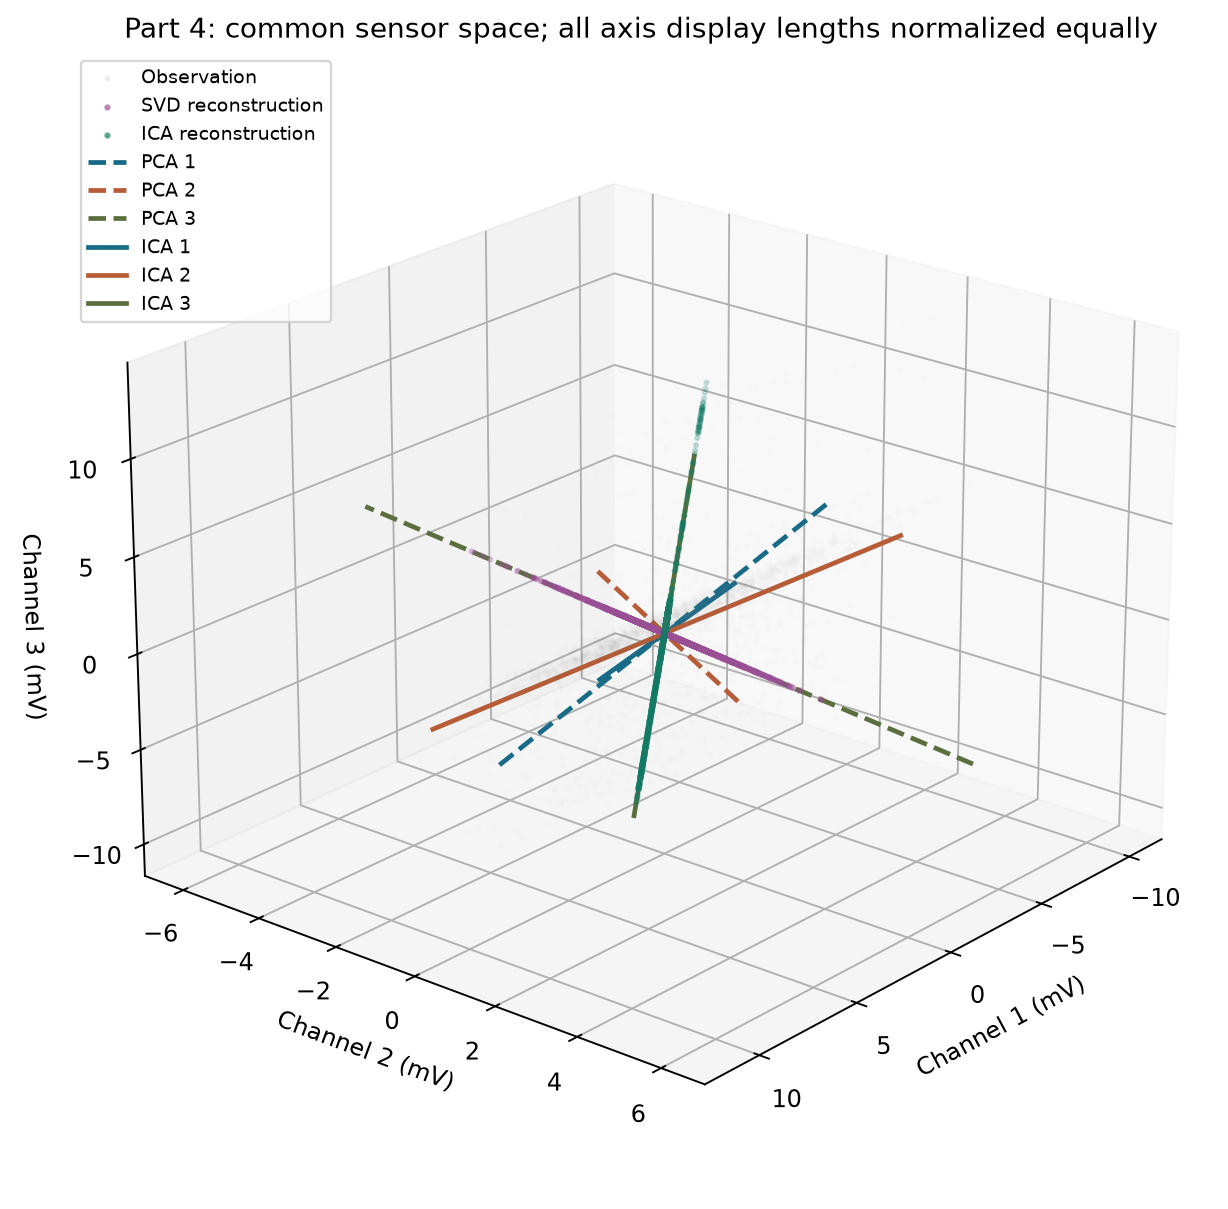
\includegraphics[width=0.7\textwidth]{fig12_geometry_comparison_3d.png}
\caption{The observations and the two reconstructions in sensor space; PCA directions are dashed and ICA directions are solid, and the display lengths are equal.}
\label{fig:geom}
\end{figure}

The direction of each vector was compared through the normalized inner product. Since the sign of an axis can be chosen oppositely, the undirected angle is reported:
\begin{equation}
\theta(\mathbf{a},\mathbf{b})=\cos^{-1}\!\left(\frac{|\mathbf{a}^{T}\mathbf{b}|}{\|\mathbf{a}\|_2\,\|\mathbf{b}\|_2}\right),\qquad 0\le\theta\le 90^\circ .
\label{eq:angle}
\end{equation}
The input of the arccosine is clipped to its valid range in the code so that rounding error cannot produce an invalid value. The reconstructions of both methods have rank one, so their scatter is linear. The line associated with SVD lies along $\mathbf{v}_3$, and the ICA line lies along $\hat{\mathbf{a}}_3$.

\begin{table}[H]
\centering
\caption{Undirected angle between the axes of each method, in degrees.}
\begin{tabular}{@{}ccc@{}}
\toprule
\textbf{Axis pair} & \textbf{PCA} & \textbf{ICA}\\
\midrule
1, 2 & 90.0000 & 62.0287\\
1, 3 & 90.0000 & 71.3380\\
2, 3 & 90.0000 & 37.6082\\
\bottomrule
\end{tabular}
\end{table}

\begin{table}[H]
\centering
\caption{Angle between the columns of $\mathbf{V}$ and the columns of the ICA mixing matrix, in degrees.}
\begin{tabular}{@{}cccc@{}}
\toprule
 & $\hat{\mathbf{a}}_1$ & $\hat{\mathbf{a}}_2$ & $\hat{\mathbf{a}}_3$\\
\midrule
$\mathbf{v}_1$ & 58.6717 & 13.5672 & 25.6578\\
$\mathbf{v}_2$ & 35.2535 & 88.4560 & 73.5767\\
$\mathbf{v}_3$ & 75.4852 & 76.5243 & 70.8559\\
\bottomrule
\end{tabular}
\end{table}

\begin{table}[H]
\centering
\caption{Column norms and the scale convention of the ICA sources.}
\begin{tabular}{@{}cccc@{}}
\toprule
\textbf{Column} & \textbf{ICA source standard deviation} & $\|\hat{\mathbf{a}}_i\|_2$ & $\|\mathbf{v}_i\|_2$\\
\midrule
1 & 1.000000 & 1.635044 & 1.000000\\
2 & 1.000000 & 2.913461 & 1.000000\\
3 & 1.000000 & 2.307861 & 1.000000\\
\bottomrule
\end{tabular}
\end{table}

The direction of the fetal ICA component and the direction of the third PCA component differ by about 70.8559 degrees. The two reconstructions are therefore not merely two scalings of one common direction. The norms of $\mathbf{V}$ are all one; the norms of $\widehat{\mathbf{A}}$ depend on the unit-variance convention of the ICA sources. Without fixing the scale convention, these norms are not a direct measure of separation quality.

\question{4-2}{Comparing the reconstructed waveform with the reference \texttt{fecg2}}

\begin{taskbox}
The fundamental question is how successful the two methods were in separation. The only way to answer it is for our knowledge of the sources and of the noise to be complete. Since simulated data are used here, our knowledge of the desired signal (fECG) and of the undesired signal (noise + mECG) is complete: for the initial data matrix $\mathbf{X}$, the desired fECG signal is given in \texttt{dat2.fecg}, a scaled version of \texttt{dat1.fecg}. By plotting the desired signal reconstructed by the SVD and ICA methods (one channel of each reconstruction) together with the ideal desired signal \texttt{fecg2}, compare their relative performance and identify the better method.
\end{taskbox}

For both methods the first channel was selected, and the same fixed reference \texttt{dat2.fecg} was used. Figure~\ref{fig:ref} separates two comparisons: the original sensor amplitude at the top and the waveform after an explicit scale adjustment at the bottom. The reference is approximately 0.8 times \texttt{dat1.fecg}, but the contribution of the same source in each sensor has a different mixing coefficient; the mismatch of raw amplitude with the reference alone is therefore not a sign of separation failure.

\begin{figure}[H]
\centering
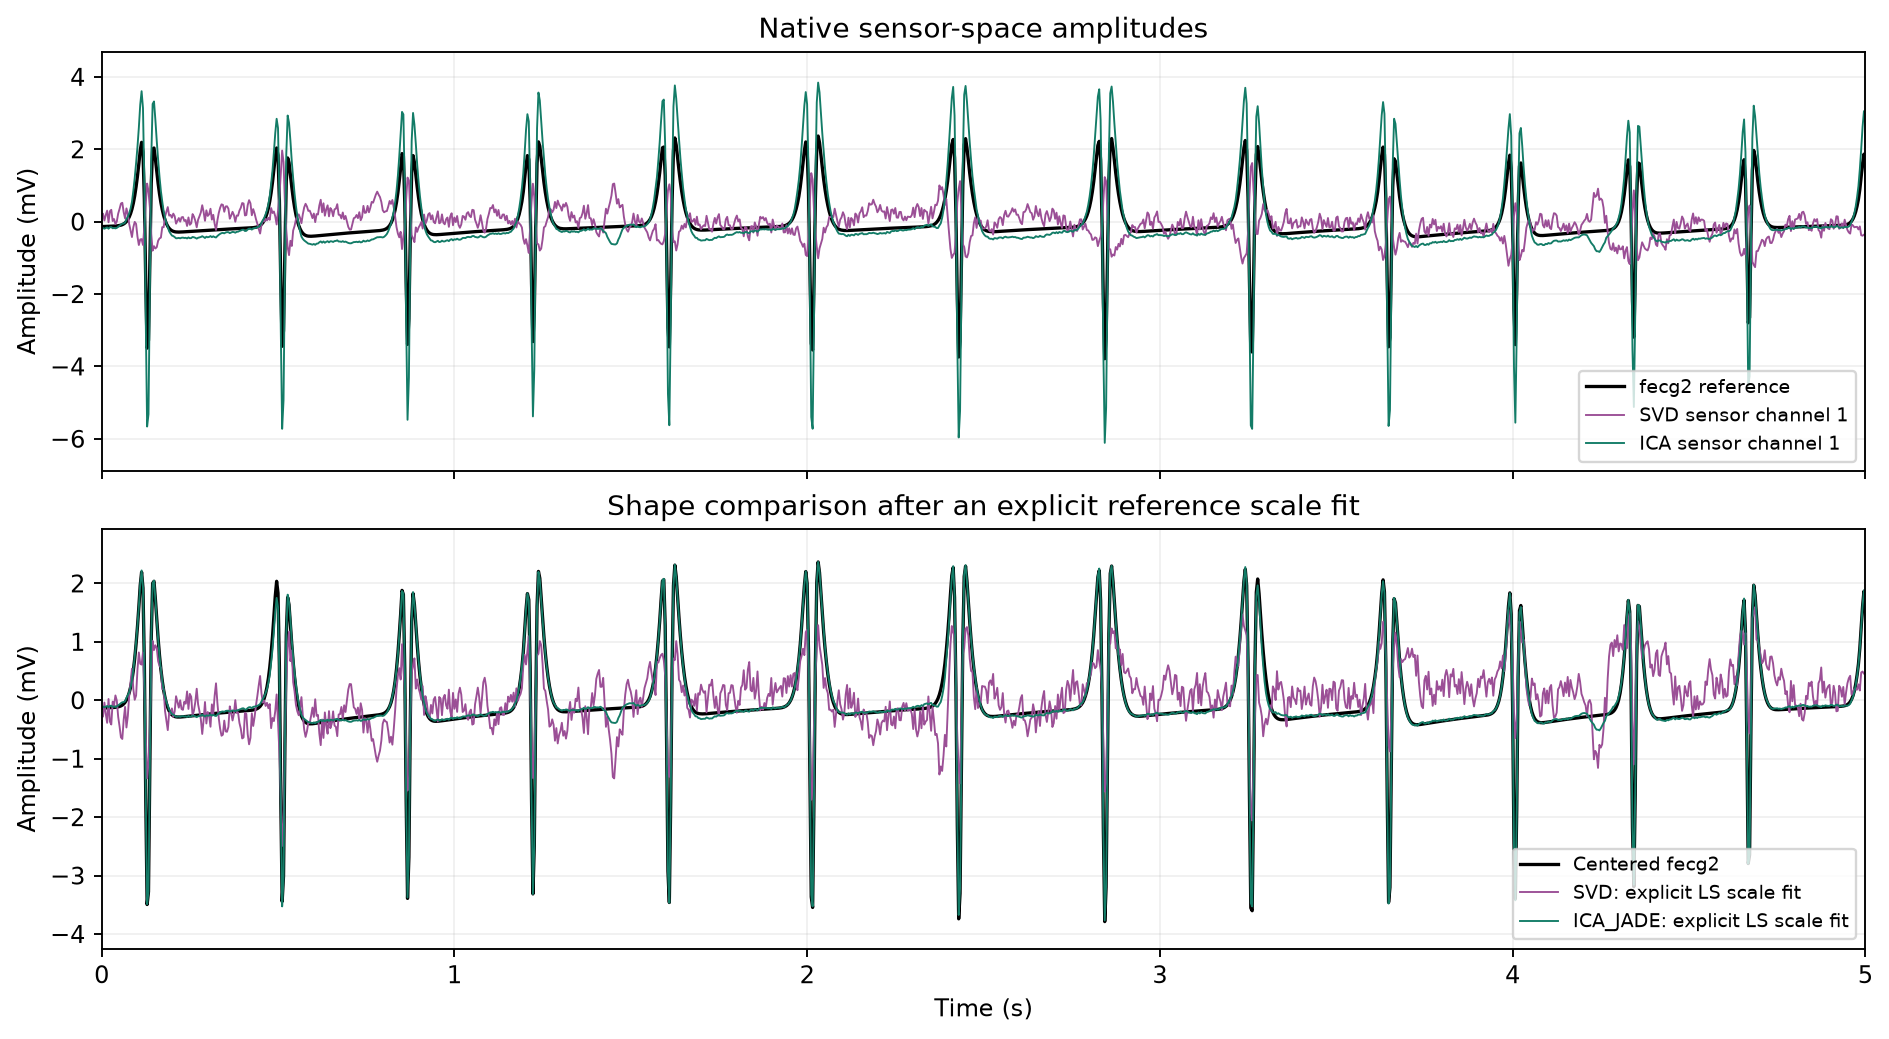
\includegraphics[width=0.95\textwidth]{fig13_reference_waveform_comparison.png}
\caption{Comparison of the first channel of the two reconstructions with the reference; top: original amplitude, bottom: after least-squares scale fitting.}
\label{fig:ref}
\end{figure}

If $\mathbf{r}$ is the centered reference and $\mathbf{y}$ the centered output, the fitting coefficient is
\begin{equation}
\alpha^{*}=\frac{\mathbf{y}^{T}\mathbf{r}}{\mathbf{y}^{T}\mathbf{y}},\qquad
\mathbf{y}_{\mathrm{aligned}}=\alpha^{*}\mathbf{y}.
\label{eq:alpha}
\end{equation}
For the first channel, $\alpha^{*}_{\mathrm{SVD}}=-1.268616$ and $\alpha^{*}_{\mathrm{ICA}}=0.616319$. These coefficients were used only in the comparison after the separation. With this convention, the ICA curve lies close to the reference, whereas deviation and oscillation remain for SVD; the better method on this data is therefore ICA.

The complementary error measures used in the table of the next question are defined with the same scale convention:
\begin{equation}
\mathrm{NRMSE}=\frac{\|\alpha^{*}\mathbf{y}-\mathbf{r}\|_2}{\|\mathbf{r}\|_2},\qquad
\mathrm{SNR}_{\mathrm{aligned}}=10\log_{10}\frac{\|\mathbf{r}\|_2^{2}}{\|\alpha^{*}\mathbf{y}-\mathbf{r}\|_2^{2}} .
\label{eq:nrmse}
\end{equation}

\question{4-3}{Correlation coefficient and numerical comparison}

\begin{taskbox}
Compute the correlation coefficient between the ideal signal \texttt{fecg2} and the signal reconstructed by the two methods (one channel of each reconstruction) with the MATLAB \texttt{corrcoef} command, and carry out the comparison.
\end{taskbox}

The correlation coefficient was computed with \texttt{numpy.corrcoef}:
\begin{equation}
\rho(\mathbf{y},\mathbf{r})=\frac{\sum_n (y_n-\bar{y})(r_n-\bar{r})}{\sqrt{\sum_n (y_n-\bar{y})^2\,\sum_n (r_n-\bar{r})^2}} .
\label{eq:rho}
\end{equation}

\begin{table}[H]
\centering
\caption{Signed correlation with the fetal reference and its absolute value.}
\begin{tabular}{@{}ccccc@{}}
\toprule
\textbf{Channel} & $\rho_{\mathrm{SVD}}$ & $\rho_{\mathrm{ICA}}$ & $|\rho_{\mathrm{SVD}}|$ & $|\rho_{\mathrm{ICA}}|$\\
\midrule
1 & $-0.674948$ &  0.997840 & 0.674948 & 0.997840\\
2 &  0.674948 &  0.997840 & 0.674948 & 0.997840\\
3 & $-0.674948$ & $-0.997840$ & 0.674948 & 0.997840\\
\bottomrule
\end{tabular}
\end{table}

In the first channel, the signed correlation coefficient of SVD is $-0.674948$ and that of ICA is $+0.997840$. The absolute value is shown to compare similarity irrespective of polarity inversion; the signed coefficient is also kept in the table. The inversion of the first SVD channel arises from the reconstruction and the sensor direction, and does not change if the signs of the SVD factors are swapped simultaneously.

\begin{figure}[H]
\centering
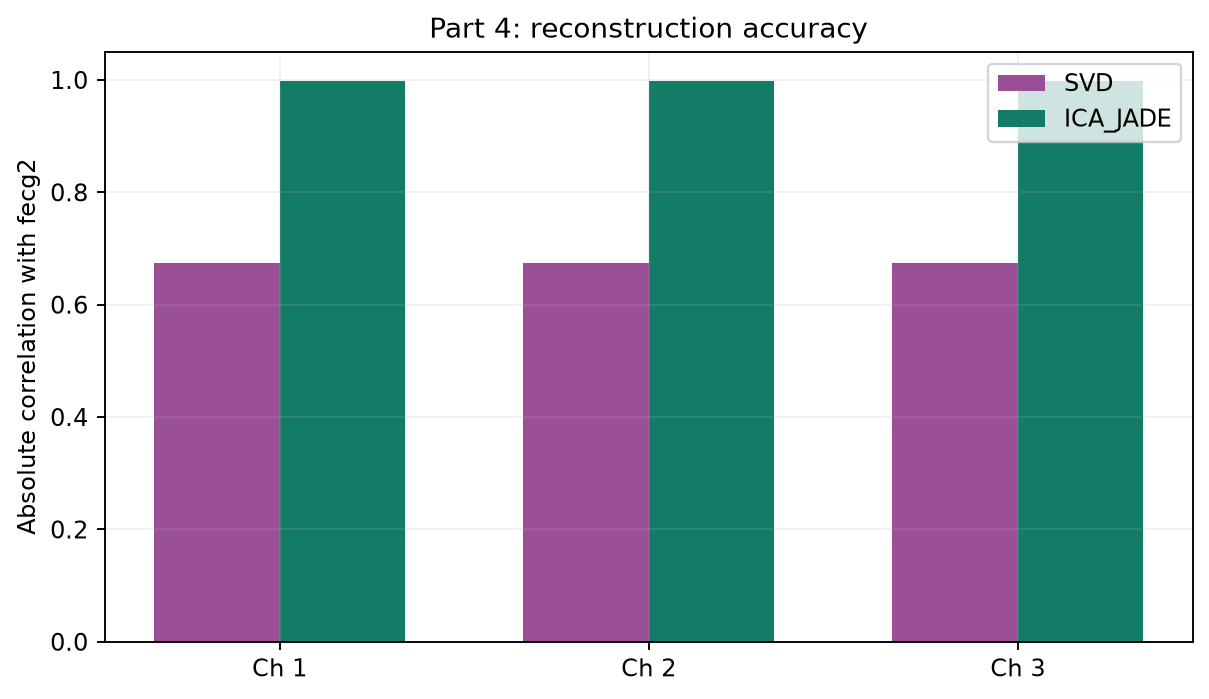
\includegraphics[width=0.62\textwidth]{fig14_correlation_bars.png}
\caption{Absolute correlation of the reconstructions with the reference in each of the three channels.}
\label{fig:corr}
\end{figure}

The equality of the absolute correlation across the channels of one method arises because the single-component reconstruction in each channel is a multiple of the same temporal signal; these three columns are not three independent validations.

\begin{table}[H]
\centering
\caption{Errors of the first channel; the scale-matched measures are computed after fitting to the reference.}
\begin{tabular}{@{}lcccc@{}}
\toprule
\textbf{Method} & \textbf{Raw MSE} & \textbf{Scale-matched MSE} & \textbf{NRMSE} & \textbf{SNR (dB)}\\
\midrule
SVD      & 1.280301 & 0.348309 & 0.737866 &  2.6405\\
ICA/JADE & 0.249628 & 0.002760 & 0.065684 & 23.6508\\
\bottomrule
\end{tabular}
\end{table}

This SNR is the ratio of the reference power to the error after scale adjustment; it is not the input SNR or the percentage of noise removed. The scale-matched MSE of ICA in this run is about 126 times smaller than that of SVD.

\question{4-4}{Final comparison, advantages and limitations}

\begin{taskbox}
Make a final comparison between the SVD and ICA methods and state the advantages and disadvantages of the two methods in general.
\end{taskbox}

\begin{table}[H]
\centering
\renewcommand{\arraystretch}{1.3}
\begin{tabularx}{\textwidth}{@{}>{\bfseries\raggedright}p{3.1cm}XX@{}}
\toprule
\textnormal{} & \textbf{SVD/PCA} & \textbf{ICA/JADE}\\
\midrule
Information used & Covariance structure and second-order statistics & In JADE, whitening and fourth-order cumulants\\
Objective & Orthogonal axes of maximum variance & Estimation of components with greater statistical independence\\
Advantage in this experiment & Simple, compact decomposition and display of the variance share & Better separation of the mother, fetus and noise in this data\\
Limitation & Decorrelation does not guarantee that a source is pure & Depends on the suitability of the mixing model and on the quality of the data and sources\\
Scale and order & Order follows the singular values; the sign of the factors is arbitrary & Order, sign and scale of the sources are ambiguous\\
Result of this run & $|\rho|\simeq 0.674948$ & $|\rho|\simeq 0.997840$\\
\bottomrule
\end{tabularx}
\end{table}

From a theoretical point of view, making the correlation zero removes only the second-order part of the dependence. Whitening can produce uncorrelated components while statistical dependence remains, which is why ICA needs a step based on independence. This explanation is consistent with the experimental result: equal source variances and orthogonal PCA components were not sufficient for the desired separation.

\begin{notebox}
\textbf{Limitations of the present evaluation.} Only one simulated 10-second record was examined. Linear separation, a sufficient number of channels and an approximation of source independence are assumed. A multi-record test, a sensitivity analysis with respect to noise, and a formal measurement of the sensitivity and positive predictive value of fetal peak detection were not performed. The final judgment of this report is therefore the waveform recovery in this same record.
\end{notebox}

\question{4-5}{The most important point learned}

\begin{taskbox}
State the most important point you learned from this experiment.
\end{taskbox}

The most important lesson is that uncorrelatedness is not equivalent to statistical independence, and a component with larger variance is not necessarily the desired signal. In the data of this experiment, all three sources of Part~1 have approximately unit variance, but their distributions and spectra differ. SVD displays them on orthogonal axes, whereas ICA, by using more statistical information, achieves a more successful separation. Moreover, judging by a nicer-looking shape alone is not enough; an independent reference, the correlation, an error with a specified scale convention and a matrix-reconstruction check must be examined together.
